%
% File acl2013.tex
%
% Contact  navigli@di.uniroma1.it
%%
%% Based on the style files for ACL-2012, which were, in turn,
%% based on the style files for ACL-2011, which were, in turn, 
%% based on the style files for ACL-2010, which were, in turn, 
%% based on the style files for ACL-IJCNLP-2009, which were, in turn,
%% based on the style files for EACL-2009 and IJCNLP-2008...

%% Based on the style files for EACL 2006 by 
%%e.agirre@ehu.es or Sergi.Balari@uab.es
%% and that of ACL 08 by Joakim Nivre and Noah Smith

\documentclass[11pt]{article}
\usepackage{acl2013}
\usepackage{times}
\usepackage{url}
\usepackage{latexsym}
\usepackage{graphicx}
\usepackage{color}
\usepackage[skip=0pt]{caption}
\usepackage{subcaption}
\usepackage{subfig}
\usepackage{pgfplotstable}
\usepackage{adjustbox}
\usepackage{booktabs}
\usepackage{amssymb}
\usepackage{amsmath}
\usepackage{enumerate}
\usepackage{paralist}
\usepackage{xspace}


\newcommand{\RQ}[1][1]{\textbf{RQ#1}\xspace}

\newcommand{\figref}[2][]{Fig#1.~\ref{#2}\xspace}
\newcommand{\tabref}[2][]{Tab#1.~\ref{#2}\xspace}

\newcommand{\lex}[1]{\textit{#1}\xspace}

\newcommand{\dataset}[1]{\texttt{#1}\xspace}
\newcommand{\EWT}{\dataset{EWT}}
\newcommand{\WSJ}{\dataset{WSJ}}
\newcommand{\Brown}{\dataset{Brown}}
\newcommand{\Reuters}{\dataset{Reuters}}
\newcommand{\MUC}{\dataset{MUC7}}

\newcommand{\method}[2][]{\ensuremath{\textsc{#2#1}}\xspace}
\newcommand{\unigram}[1][]{\method{Unigram}}
\newcommand{\brown}[1][]{\method[\ensuremath{_{#1}}]{Brown}}
\newcommand{\CW}[1][]{\method[#1]{CW}}
\newcommand{\CBOW}[1][]{\method[#1]{CBOW}}
\newcommand{\Skipgram}[1][]{\method[#1]{Skip-gram}}
\newcommand{\Glove}[1][]{\method[#1]{Glove}}
\newcommand{\withup}{\method{+UP}}

\newcommand{\task}[1]{\textsf{#1}\xspace}
\newcommand{\pos}{\task{POS-tagging}}
\newcommand{\chunking}{\task{Chunking}}
\newcommand{\ner}{\task{NER}}
\newcommand{\mwe}{\task{MWE}}

\newcommand{\evmeasure}[1]{\textsc{#1}\xspace}
\newcommand{\accuracy}{\evmeasure{Acc}}
\newcommand{\fscore}{\evmeasure{F1}}


\newcommand{\best}[1]{\textbf{#1}}

\newcommand{\ctx}{\ensuremath{\text{ctx}}}


\hyphenation{an-aly-sis}
\hyphenation{an-aly-ses}
\hyphenation{an-aly-ser}

\title{Big Data Small Data, In Domain Out-of Domain, Known Word Unknown
  Word: The Impact of Word Representation on Sequence Labelling Tasks}

\author{A Anonymous 
   \\%NICTA / Locked Bag 8001, \\ Canberra ACT 2601, Australia \\
   \\ %The Australian National University\\
   \\ %University of Canberra \\
  \\ % {\tt \small{@nicta.com.au}} \\
\And
  B Anonymous
   \\%NICTA / Locked Bag 8001, \\ Canberra ACT 2601, Australia \\
   \\%The Australian National University\\ \\
   \\ %{\tt \small{@nicta.com.au}} \\
}

\date{}

% Max 8 pp.

\begin{document}


\maketitle


\begin{abstract} 
  Word embeddings -- distributed word representations that can be
  learned from unlabelled data -- have been shown to have high utility
  in many natural language processing applications. 
  In this paper, we perform an extrinsic evaluation of five popular word
  embedding methods in the context of four sequence labelling tasks:
  POS-tagging, syntactic chunking, NER and MWE identification.
  A particular focus of the paper is analysing the effects of task-based
  updating of word representations.
  We show that when using word embeddings as features, as few as
  several hundred training instances are sufficient to achieve competitive
  results, and that word embeddings lead to improvements over OOV words
  and out of domain.
  Perhaps more surprisingly, our results indicate there is little
  difference between the different word embedding methods, and that simple
  Brown clusters are often competitive with word embeddings across all
  tasks we consider. 
\end{abstract}

\newcommand{\gabi}[1]{\textcolor{blue}{#1}}
\newcommand{\tim}[1]{\textcolor{red}{#1}}
\newcommand{\lizhen}[1]{\textcolor{green}{#1}}
\newcommand{\nss}[1]{\textcolor{magenta}{#1}}

\section{Introduction}

Recently, distributed word representations have grown to become a
mainstay of natural language processing (NLP), and been show to have
empirical utility in a myriad of tasks
\cite{Collobert2008,turian2010word,baroni:2014,Andreas:Klein:2014}.  The
underlying idea behind distributed word representations is simple: to
map each word $w$ in our vocabulary $V$ onto a continuous-valued vector
of dimensionality $d \ll |V|$.  Words that are similar
(e.g., with respect to syntax or lexical semantics) will ideally be mapped to
similar regions of the vector space, implicitly supporting both
generalisation across in-vocabulary (IV) items, and countering the
effects of data sparsity for low-frequency and out-of-vocabulary (OOV)
items.

Without some means of automatically deriving the vector representations
without reliance on labelled data, however, word embeddings would have
little practical utility. Fortunately, it has been shown that they can
be ``pre-trained'' from unlabelled text data using various algorithms 
to model the distributional hypothesis (i.e., that
words which occur in similar contexts tend to be semantically
similar). Pre-training methods have been refined considerably in recent
years, and scaled up to increasingly large corpora.

As with other machine learning methods, it is well known that the
quality of the pre-trained word embeddings depends heavily on factors
including parameter optimisation, the size of the training data, and the
fit with the target application. For example, \newcite{turian2010word}
showed that the optimal dimensionality for word embeddings is task-specific.  
One factor which has received relatively little attention in
NLP is the effect of ``updating'' the pre-trained word embeddings as
part of the task-specific training, based on self-taught
learning~\cite{raina2007self}.  Updating leads to word
representations that are task-specific, but often at the cost of
over-fitting low-frequency and OOV words.


In this paper, we perform an extensive evaluation of five word embedding
approaches under fixed experimental conditions, applied to four sequence
labelling tasks: POS-tagging, full-text chunking, named entity
recognition (NER), and multiword expression (MWE) identification. In
this, we explore the following research questions:
\begin{compactenum}[\bf RQ1:]
\item are word embeddings better than baseline approaches of one-hot
  unigram features and Brown clusters?
\item do word embeddings require less training data (i.e.\ generalise
  better) than one-hot unigram features?
\item what is the impact of updating word embeddings in sequence
  labeling tasks, both empirically over the target task and
  geometrically over the vectors?
\item what is the impact of word embeddings (with and without
  updating) on both OOV items (relative to the training data) and
  out-of-domain data?
\item overall, are some word embeddings better than others in a sequence
  labelling context?
\end{compactenum}



\section{Word Representations}
\label{wordrep} 

\subsection{Types of Word Representations}

\newcite{turian2010word} identifies three varieties of word
representations: \textit{distributional}, \textit{cluster-based}, and
\textit{distributed}.

\textit{Distributional representation} methods map each word $w$ to a
context word vector $\mathbf{C}_w$, which is constructed directly from
co-occurrence counts between $w$ and its context words.  The learning
methods either store the co-occurrence counts between two words $w$ and
$i$ directly in
$C_{wi}$~\cite{sahlgren2006word,turney2010frequency,honkela1997self} or
project the concurrence counts between words into a lower dimensional
space~\cite{vrehuuvrek2010software,lund1996producing}, using
dimensionality reduction techniques such as SVD~\cite{dumais1988using} and
LDA~\cite{blei2003latent}.

\textit{Cluster-based representation} methods build clusters of words by applying either soft or hard clustering algorithms~\cite{lin2009phrase,li2005semi}. Some of them also rely on a co-occurrence matrix of words~\cite{pereira1993distributional}. The Brown clustering algorithm~\cite{Brown92class-basedn-gram} is the best-known method in this category.

\textit{Distributed representation} methods usually map words into dense,
low-dimensional, continuous-valued vectors, with $\mathbf{x} \in
R^d$, where $d$ is referred to as the word dimension.

\subsection{Selected Word Representations}

Over a range of sequence tagging tasks, we evaluate five methods for
inducing word representations: Brown clustering
\cite{Brown92class-basedn-gram} (``\brown''), the neural language model
of Collobert \& Weston (``\CW'')~\cite{collobert2011natural}, the
continuous bag-of-words model (``\CBOW'')~\cite{Mikolov13}, the continuous
skip-gram model (``\Skipgram'')~\cite{Mikolov13NIPS}, and Global vectors
(``\Glove'')~\cite{pennington2014glove}. With the exception of \CW, all have
have been shown to be at or near state-of-the-art in recent empirical
studies~\cite{turian2010word,pennington2014glove}. \CW is included
because it was highly influential in earlier research, and the pre-trained embeddings are
still used to some degree in NLP. The training of these word
representations is unsupervised: the common underlying idea is to
predict occurrence of words in the neighbouring context. Their training
objectives share the same form, which is a sum of local training factors
$J(w, \text{ctx}(w))$,  
\begin{displaymath}
  L = \sum_{w \in V} J(w, \ctx(w))
\end{displaymath}

where $V$ is the vocabulary of a given corpus, and $\ctx(w)$ denotes the
local context of word $w$.
The local context of a word can either be its previous $k$ words, or the
$k$ words surrounding it. 
Local training factors are designed to capture the relationship between
$w$ and its local contexts of use, either by predicting $w$
based on its local context, or using $w$ to predict the
context words. Other than \brown, which utilises a cluster-based
representation, all the other methods employ a distributed representation.

The starting point for \CBOW and \Skipgram is to employ softmax to predict word occurrence:
\begin{displaymath}
  J(w, \ctx(w)) = - \log \left( \frac{\exp(\mathbf{v}_w^{\text{T}} \mathbf{v}_{\ctx(w)})}{ \sum_{j \in V} \exp(\mathbf{v}_j^{\text{T}} \mathbf{v}_{\ctx(w)})} \right)
\end{displaymath}
where $\mathbf{v}_{\ctx(w)}$ denotes the distributed representation of
the local context of word $w$. \CBOW derives $\mathbf{v}_{\ctx(w)}$
based on averaging over the context words. That is, it estimates the
probability of each $w$ given its local
context. In contrast, \Skipgram applies softmax to each context word of
a given occurrence of word $w$. In this case, $\mathbf{v}_{\ctx(w)}$ corresponds to the
representation of one of its context words. This model can be characterised as
predicting context words based on $w$. In practice, softmax is
too expensive to compute over large corpora, and thus~\newcite{Mikolov13NIPS} use
hierarchical softmax and negative sampling to scale up the training.

\CW considers the local context of a word $w$ to be $m$ words to the left
and $m$ words to the right of $w$. The concatenation of the embeddings of
$w$ and all its context words are taken as input to a neural network
with one hidden layer, which produces a higher level representation
$f(w) \in R^d$. Then the learning procedure replaces the embedding of
$w$ with that of a randomly sampled word $w'$ and generates a second
representation $f(w') \in R^d$ with the same neural network. The
training objective is to maximise the difference between them:
\begin{displaymath}
J(w, \ctx(w)) = \max (0, 1 - f(w) + f(w'))
\end{displaymath}
This approach can be regarded as negative sampling with only one negative example.

\Glove assumes the dot product of two word embeddings should be similar
to the logarithm of the co-occurrence count $X_{ij}$ of the two
words. As such, the local factor $J(w, \ctx(w))$ becomes:
\begin{displaymath}
g(X_{ij}) (\mathbf{v}_i^{\text{T}} \mathbf{v}_j + b_i + b_j - \log(X_{ij}))^2
\end{displaymath}
where $b_i$ and $b_j$ are the bias terms of words $i$ and $j$,
respectively, and $g(X_{ij})$ is a weighting function based on the
co-occurrence count. This weighting function controls the degree of
agreement between the parametric function $\mathbf{v}_i^{\text{T}}
\mathbf{v}_j + b_i + b_j $ and $\log(X_{ij})$. Frequently co-occurring
word pairs will be larger weight
%\nss{i think you mean the weight  will be larger? or there will be more parameters?} 
than infrequent
pairs, up to a threshold.

\brown partitions words into a finite set of word classes $V$. The
conditional probability of seeing the next word is defined to be:
\begin{displaymath}
p(w_k | w_{k - m}^{k -1}) = p(w_k | h_k) p(h_k | h_{k - m}^{k -1})
\end{displaymath}
where $h_k$ denotes the word class of the word $w_k$, $w_{k - m}^{k -1}$
are the previous $m$ words and $h_{k - m}^{k -1}$ are their respective
word classes. Then $J(w, \text{ctx}(w)) = - \log p(w_k | w_{k - m}^{k
  -1}) $. Since there is no tractable method to find an optimal
partition of word classes, the method uses only a bigram class model, and utilises hierarchical clustering as an approximation method to find a sufficiently good partition of words. 



\subsection{Building Word Representations}
\label{buildingWordRep}

For a fair comparison, we train \brown, \CBOW, \Skipgram, and \Glove on
a fixed corpus, comprised of freely available corpora, as detailed in
\tabref{wordEmbedCorpora}. The joint corpus was preprocessed with the
Stanford CoreNLP sentence splitter and tokeniser. All consecutive digit
substrings were replaced by NUM\textit{f}, where \textit{f} is the
length of the digit substring (e.g., \lex{10.20} is replaced by
\lex{NUM2.NUM2}. Due to the computational complexity of the
pre-training, for \CW, we simply downloaded the pre-compiled embeddings from:
\url{http://metaoptimize.com/projects/wordreprs}.

\begin{table}[t]
\centering
\begin{tabular}{lrr}
\hline
\textbf{Data set} & \multicolumn{1}{c}{\textbf{Size}} & \multicolumn{1}{c}{\textbf{Words}} \\ \hline
UMBC 	& 48.1GB & 3G \\
One Billion 	& 4.1GB & 1G  \\
English Wikipedia & 49.6GB & 3G \\ \hline
\end{tabular}
\caption{Corpora used to pre-train the word embeddings}
\label{wordEmbedCorpora}
\end{table}

The dimensionality of the word embeddings and the size of the context
window are the key hyperparameters when learning distributed
representations. We use all combinations of the following values to
train word embeddings on the combined corpus:
\begin{itemize}
\item \textbf{Embedding dim.\ $d \in \{25, 50, 100, 200\}$}
\item \textbf{Context window size $m \in \{1, 5, 10\}$}
\end{itemize}
\brown requires only the number of clusters as a hyperparameter. We
perform clustering with $b \in \{250, 500, 1000, 2000, 4000\}$ clusters.
%
%
%Based on the idea that a word is characterized by the company it keeps \cite{firth1957}, 
%distributed word representation methods represent a given word as a continuous vector, which consists of the most frequent contexts of that given word in a big corpus.
%Therefore, similar words have a similar vector representation.
%
%Traditionally, the estimation of the vectors is done by initializing the vectors with co-occurrences counts. More recently, the vectors are learned in a supervised way, where
%the weights in the vectors are set to maximize the probability of the context in which the word is observed in the corpus. 
%Note that the method does no require an annotated corpus since the contexts windows used for training are extracted from unannotated data.
%
%More formally, learning a word vector $W: words \rightarrow \mathbb{R}^n$ is parametrized function that maps
%words to high-dimensional vectors, where $W$ is initialized to have random vectors for each word and learn to have meaningful vectors to perform same task.
%
%Learning the word vectors can be carry out with different models architectures. 
%In this paper, we evaluated five different word embeddings learning algorithms, which are the following: 
% 
%\begin{itemize}
%\item[-] Brown cluster \cite{Brown92class-basedn-gram}
%\item[-] CBOW \cite{Mikolov13NIPS}
%\item[-] Glove \cite{pennington2014glove}
%\item[-] Neural language model \cite{collobert2011natural}
%\item[-] Skip-Gram \cite{Mikolov13}
%\end{itemize}
%
%The above methods were chosen because they are recent
%state-of-the-art word embedding learning methods and because their software is
%available and all of them are neural networks architectures.
%The first method (Brown clusters) was selected as a benchmark word representation, which makes use of hard word clusters rather than a distributed representation.
%
%Skip-Gram \cite{Mikolov13} is a neuronal network language model, but it does not have a hidden layer, and 
%instead predicting the target word, it predicts the context given the target word.
%These embeddings are faster to train than other neuronal embeddings.
%(and does not involve dense matrix multiplication).
%
%The CBOW \cite{Mikolov13NIPS} model learns to predict the word in the middle of a symmetric window based on the sum of the vector representations of the words in the window.
%
%GloVe \cite{pennington2014glove} is essentially a log-bilinear model with a weighted least-squares objective. The main intuition underlying the model is the simple observation that ratios of word-word co-occurrence probabilities have the potential for encoding some form of meaning.
%
%%One of the benefits of neuronal networks are able to learn ways of representing the data automatically,



%%% Local Variables: 
%%% mode: latex
%%% TeX-PDF-mode: t 
%%% TeX-master: "WordEmbEvaluation"
%%% End: 

\section{Sequence Tagging Tasks}
\label{sec:SeqTagging}
We evaluate different word representations in four different sequence tagging tasks: POS-tagging, chunking, NER and MWE identification. 
For the POS-tagging, chunking and MWE tasks, we used the same features as the state-of-the-art approaches,  \newcite{collobert2011natural}, \newcite{turian2010word} and ~\newcite{mwecorpus}, respectively. 
For the NER, we used the same feature space as in~\newcite{turian2010word}, except for the previous two predictions.

For each sequence tagging task, we feed learned word representations into a first order linear-chain graph
transformer~\cite{collobert2011natural}, and trained them by using the online learning algorithm
AdaGrad~\cite{duchi2011adaptive}.
For each model taking distributed word representations as word features, we consider two settings: 

\begin{small}
\begin{itemize}
\item[-] Graph transformer \textit{does not} fine tune word representations during training (this is equivalent to a linear-chain CRF);
\item[-] Graph transformer fine tunes the word representations during training.
\end{itemize}
\end{small}

We consider also CRF models with hand-crafted features, which use one-hot representation for each unigram.

We split the task specific corpus into a training set, validation set, and a test set (see Table \ref{datasplit}). If a corpus already provides fixed splits, we reuse them. For POS-tagging and NER, we also evaluated the models with a out-of-domain corpus (English Web-Treebank and MUC-7, respectively), which has similar annotation schema as the respective training corpus.

\begin{table*}
\caption{Datasets splits and feature space for each sequence tagging task.}
\begin{small}
\begin{tabular}{lllp{3.cm}ll}
\hline
			& \textbf{Training set} & \textbf{Validation set} & \textbf{\textit{in-domain} Test set} & \textbf{\textit{out-of-domain} Test set} \\ \hline
\textbf{POS-Tagging} & 0-18 WSJ & 19-21 WSJ & 22-24 of WSJ & English Web-Treebank  \\
\textbf{Chunking} & WSJ & 1000 sentences WSJ & CoNLL-2000 & Brown corpus \\
\textbf{NER} & CoNLL-2003 train set & CoNLL-2003 dev. set & CoNLL-2003 test set & MUC7  \\
\textbf{MWE} & 500 documents from & 100 documents from & 123 documents & - \\
\hline
\end{tabular}
\label{datasplit}
\end{small}
\end{table*}


In order to have fair and reproducible experimental results, we tuned the hyperparameters with random search~\cite{bergstra2012random}. 
We randomly sampled 50 distinct hyperparameter sets with the same random seed for the models that do not update word embeddings, and sampled 100 distinct hyperparameter sets for the models that update word embeddings. 
For each set of hyperparameters, we train a model on its training set and pick up the best one based on its performance on its validation set~\cite{turian2010word}. 
Note that, we also consider word vector size and context window size of distributed word representation, and number of clusters of brown clustering as the hyperparameters.
This is achieved by mapping each possible hyperparameter combination to the word representation files trained with these parameters. 

However, for the models that update word representations, we always found under-performed hyperparameters after trying out all hyperparameter combinations, because they have more hyperparameters than the models that do not update word representations. Then, for each distributed word representations, we reuse all hyperparameters of the models that do not update word representations, only tune the hyperparameters of AdaGrad for the word representation layer. This method requires only 32 additional runs for each model updating embeddings and achieves consistently better results than 100 random draws.

The final evaluation is carried out in a semi-supervised setting. We split the training set into 10 partitions at log scale. That means, the second smallest partition will be twice the size of the smallest partition. We created 10 training sets with incremental size by merging these partitions from the smallest one to the largest one, and each of them on the same designated test sets. 

We adopted the most commonly used F1 measure as the evaluation metric for all tasks except POS tagging, for which we use per-word accuracy. In order to evaluate model performance on out-of-vocabulary (unknown) words, we reported also the accuracy for the words that do not occur in the training set.

In addition, we also set up experiments to verify if CRF/graph transformer requires different feature design for different kinds of pre-trained word embeddings. This is achieved by adding a hidden layer between CRF and distributed word representations. For each context word, the hidden layer computes the element-wise multiplication of its embedding with the embedding of the current word embedding, and the representation of current word stays the same. The results of this approach are not plotted because this method leads only to marginal improvement.

%\subsection{POS tagging} We could choose one of the options. \subsubsection{Option 1} Almost the same setting as~\cite{collobert2011natural}, except adding one more test set.
% \noindent Training set: 0-18 of WSJ.
% \noindent Validation set: 19-21 of WSJ.
% \noindent Test set: 22-24 of WSJ, and English Web Treebank. We report model performances on these two test sets respectively.
% \noindent Feature space: the same set as in~\cite{collobert2011natural}

% \subsection{Chunking} The same setting as~\cite{turian2010word}\\
% \noindent Training set: WSJ train set.
% \noindent Validation set: Randomly sampled 1000 sentences from the train set for development.
% \noindent Test set: CoNLL2000 test set.
% \noindent Feature space: the same set as in~\cite{turian2010word}

% \subsection{MWE Identification} Training set: randomly sampled 500 documents from Nathana��s corpus. 
% \noindent Validation set: randomly sampled 100 documents from Nathana��s corpus.
% \noindent Test set: remaining 123 documents from Nathana��s corpus..
% \noindent Feature space: the same set as in~\cite{mwecorpus}

%\subsection{Named entity recognition} Training set: CoNLL03 train set.
% \noindent Validation set: CoNLL03 development set.
% \noindent Test set: CoNLL03 test set and MUC7. We report model performances on these two test sets respectively.
% \noindent Feature space: the same set as in~\cite{turian2010word}
\section{Experimental Results and Discussion}

%%%% BECHMARKS
\begin{table*}
\caption{Benchmark results vs. our best results for in-domain and out-of-domain test sets (Acc. refers to Accuracy; F1 refers to F1-measure).}
\begin{center}
\begin{small}
\begin{tabular}{llll}
\hline
\textbf{Task} & \textbf{Benchmark} & \textbf{\textit{in-domain} Test set} & \textbf{\textit{out-of-domain} Test set} \\ \hline
POS-Tagging & (Acc.) 0.972 \cite{Toutanova:2003} & 0.959 (skip-gram negsam+up) & 0.910 (skip-gram negsam+noup)\\ 
Chunking & (F1) 0.942 \cite{Sha:2003} & 0.938 (Brown cluster v2000) & 0.676 (glove+noup)\\  
NER & (F1) 0.893 \cite{Ando:2005} & 0.868 (skip-gram negsam+noup) & 0.736 (skip-gram negsam+noup) \\  
MWE & (F1) 0.625 \cite{Schneider+:2014} & 0.654 (cw+up) & - \\ 
\hline
\label{benchmark}
\end{tabular}
\end{small}
\end{center}
\end{table*}

%%%%%%%%%%%%%%%%%%%%%%%%%%%%
%%% HEATMAPS 
\begin{figure*}
\caption{Best results for each method for POS-Tagging, Chunking, NER and MWE identification. The x-axis correspond to the different word embeddings methods and the y-axis to the 10 training partitions at log scale. Green color stand for high performance, while red color stands for low performance. The methods are in chronological order; wherein the suffix \textit{up} stands for \textit{updated or fine-tuned features}, and \textit{noup} stands for \textit{no-updated} features.}
\centering
\begin{subfigure}{7cm}
	\centering
    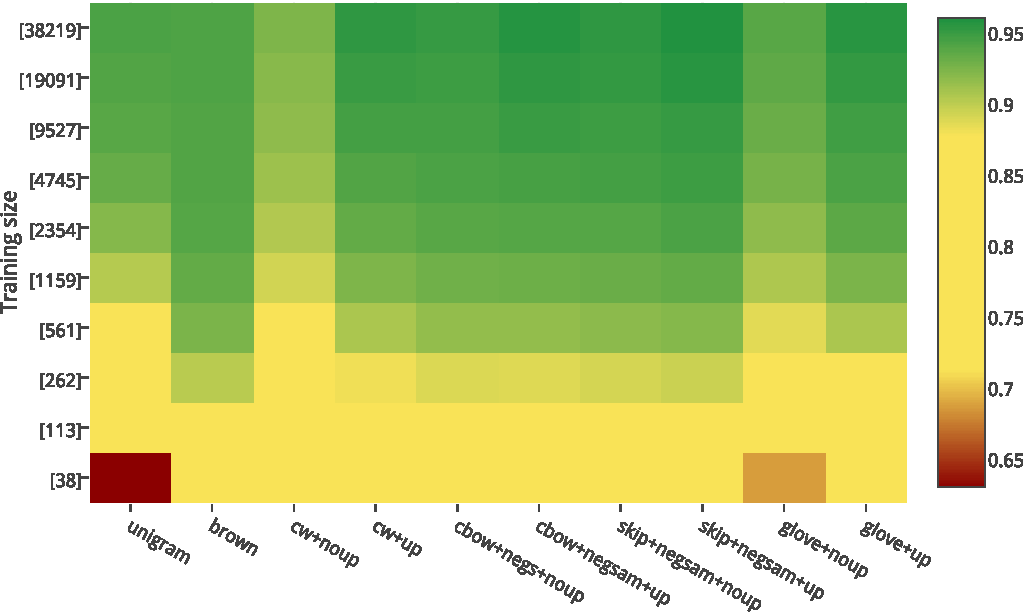
\includegraphics[scale=0.4]{plots/map-pos-color-invert}    	
	\subcaption{POS-Tagging Accuracy}	
	\label{pos}
\end{subfigure}
\begin{subfigure}{7cm}
	\centering
    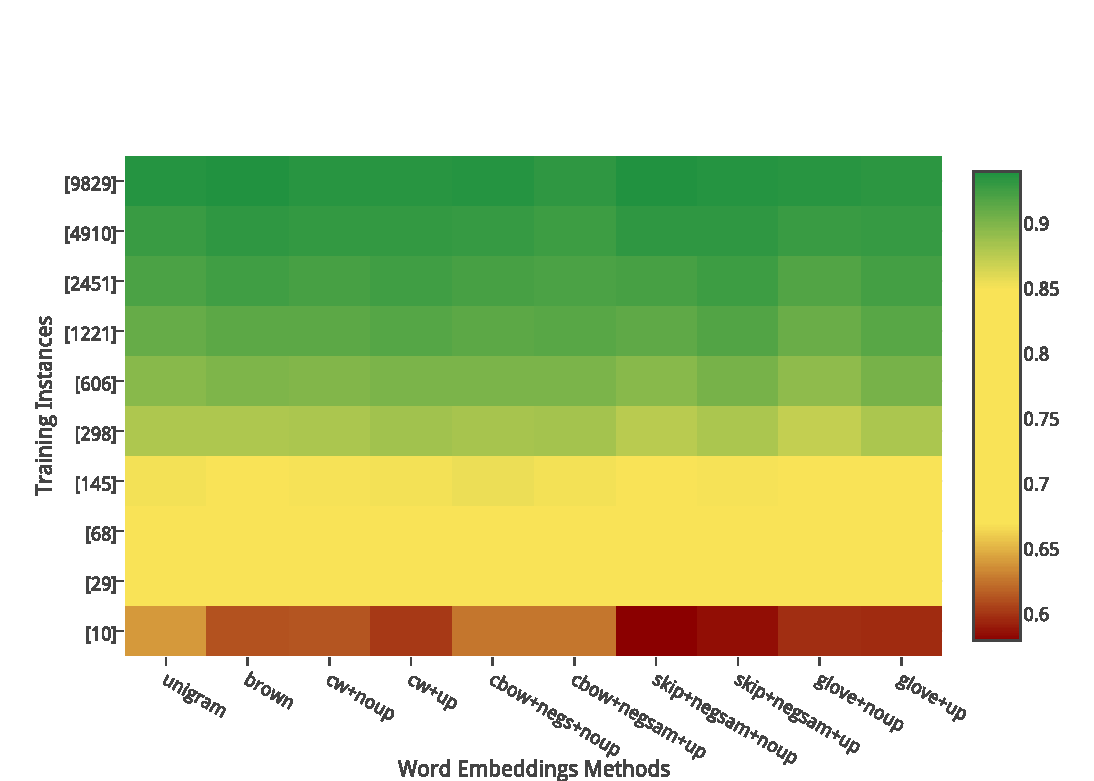
\includegraphics[scale=0.4]{plots/map-chunk-color-invert}
	\subcaption{Chunking F1-Measure}	
	\label{chu}
\end{subfigure}
%\\[-2ex]  %%<-- in this line
\begin{subfigure}{7cm}
	\centering
    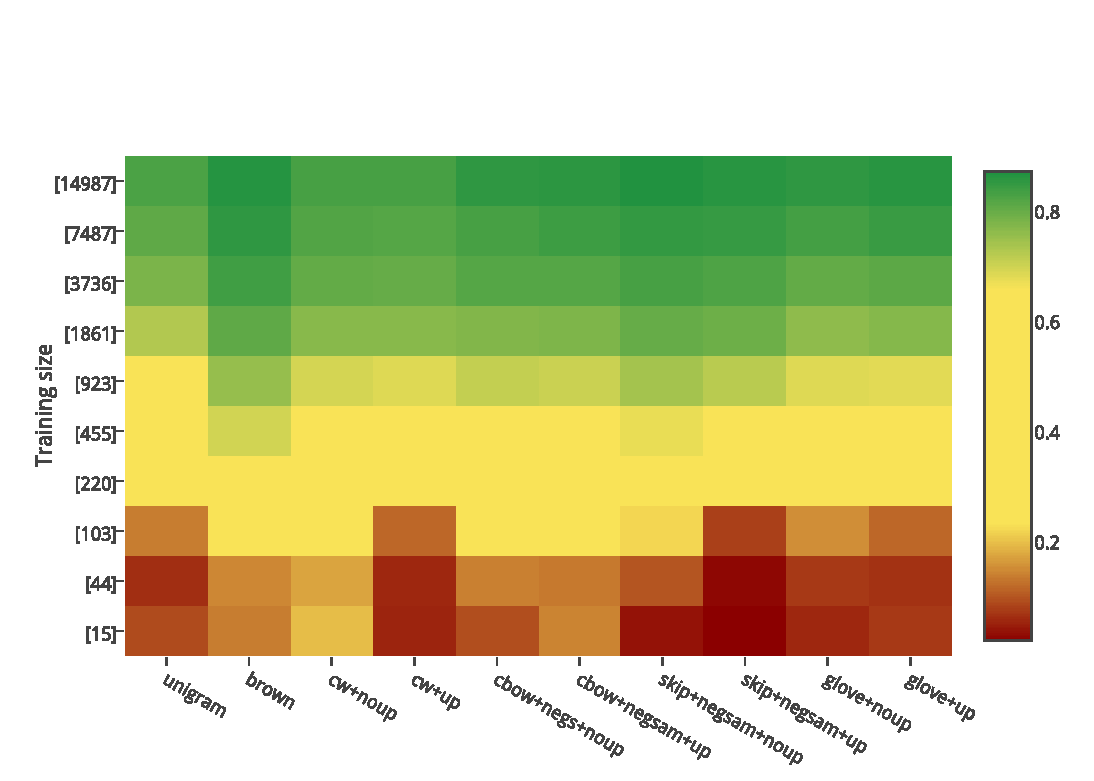
\includegraphics[scale=0.4]{plots/map-ner-color-invert}    	
	\subcaption{NER F1-Measure}	
	\label{ner}
\end{subfigure}
\begin{subfigure}{7cm}
	\centering
    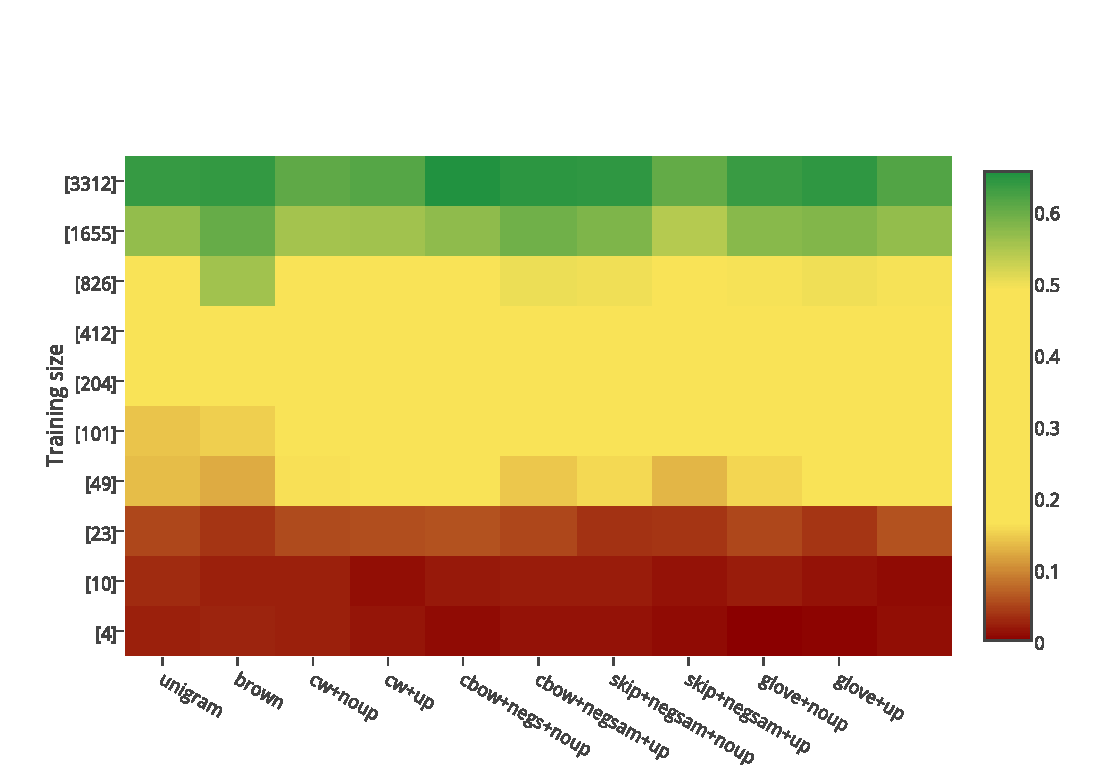
\includegraphics[scale=0.4]{plots/map-mwe-color-invert}
	\subcaption{MWEs F1-Measure}		
	\label{mwe}
\end{subfigure}
\label{fig:heatmaps}
\end{figure*}


%%%%%%%%%%%%%%%%%%%%%%%%%%%%
%%% Vector fields
% POS
\begin{figure*}
\caption{Updated vs. no-updated word representations for POS-tagging and chunking using skip-gram}
\centering
\begin{subfigure}[b]{0.48\textwidth}
	\centering
    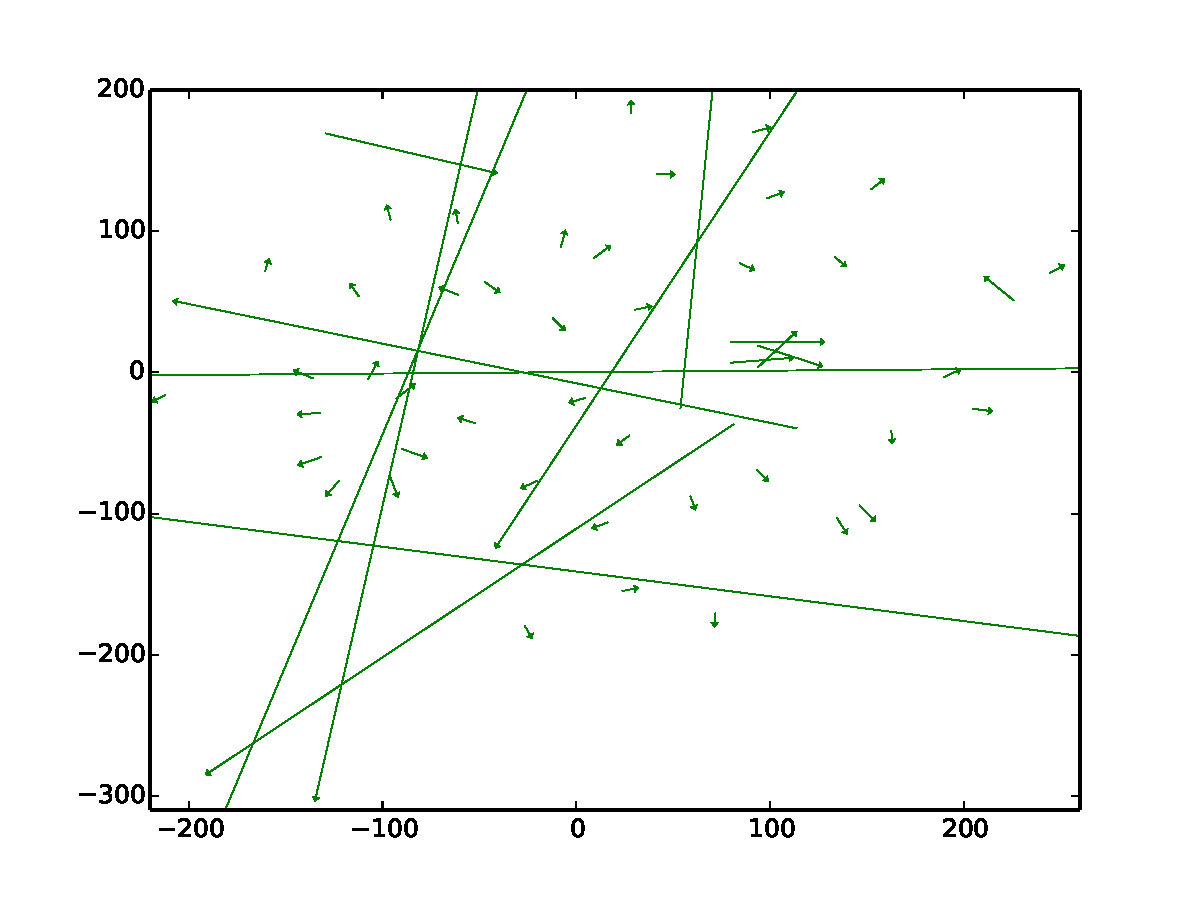
\includegraphics[width=\textwidth]{plots/vectorField/Lizhen/scaled/Lizhen_skip_chunking}
	\label{fig:skipChu}
	\subcaption{Chunking}	
\end{subfigure}
\begin{subfigure}[b]{0.48\textwidth}
	\centering
    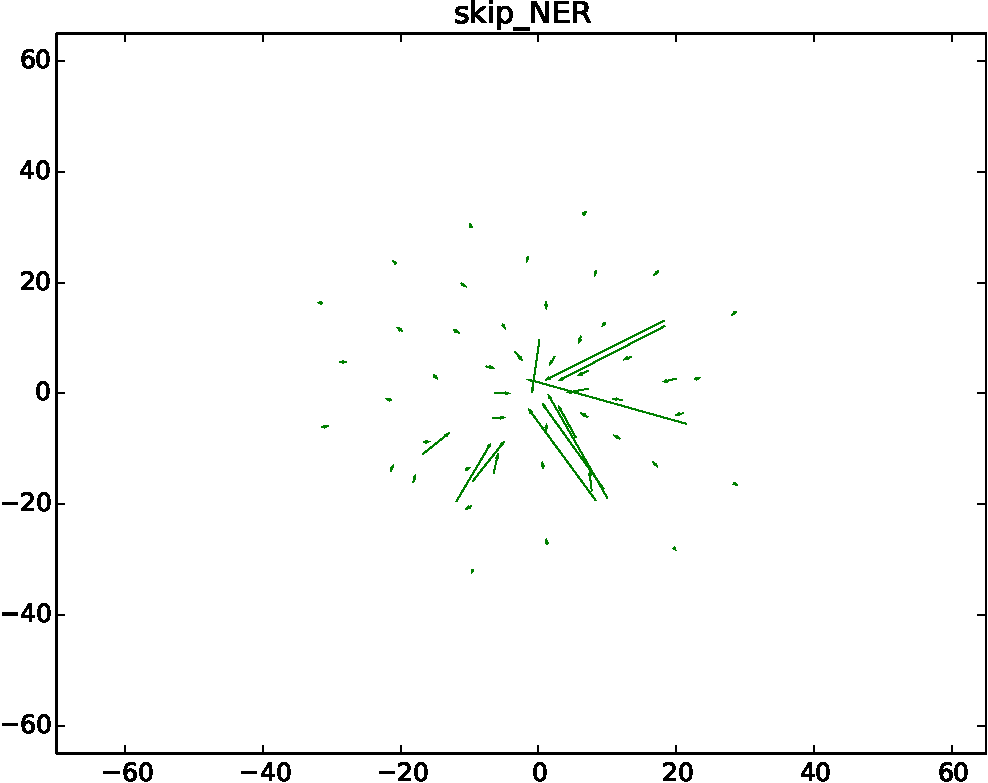
\includegraphics[width=\textwidth]{plots/vectorField/Lizhen/scaled/Lizhen_skip_NER}    	
	\label{fig:skippos}
	\subcaption{NER}	
\end{subfigure}
%\begin{subfigure}[b]{0.48\textwidth}
%	\centering
%   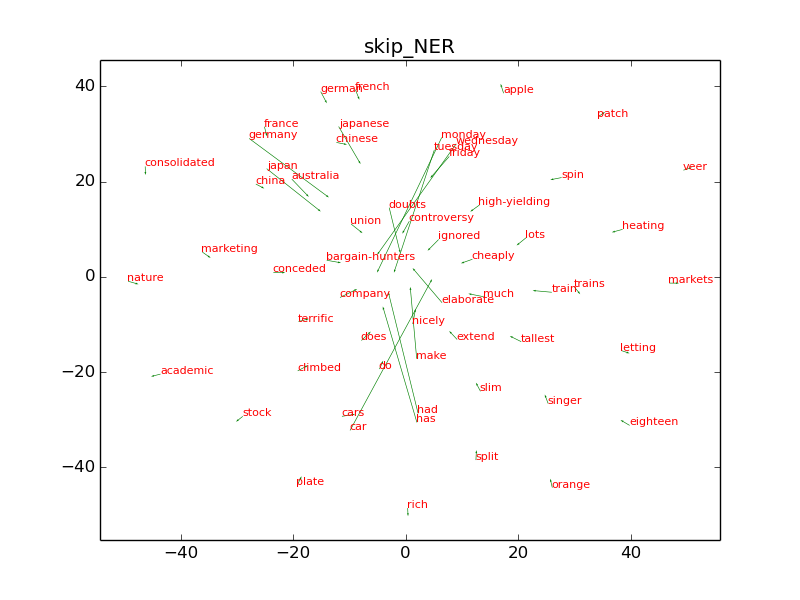
\includegraphics[width=\textwidth]{plots/vectorField/skip_NER.png}
%	\label{fig:skipner}
%	\subcaption{}	
%\end{subfigure}
%%\begin{subfigure}{6cm}
%	\centering
 %   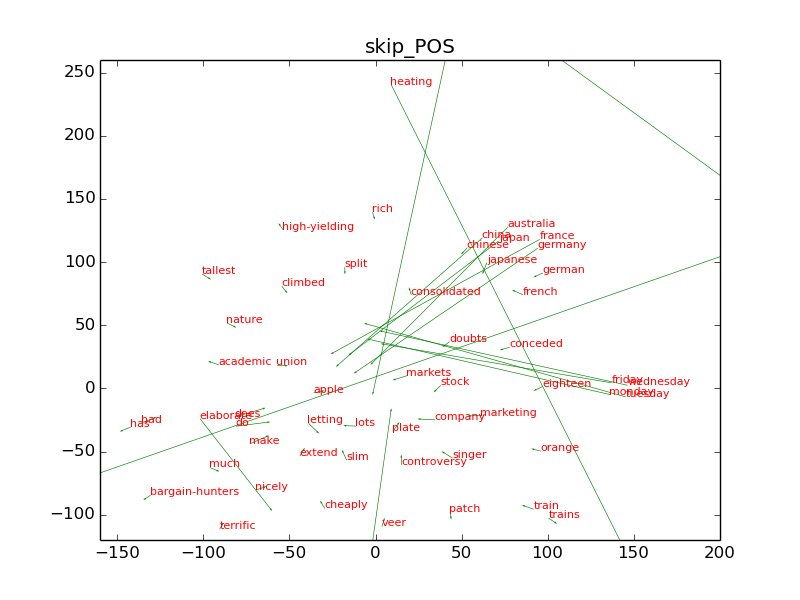
\includegraphics[scale=0.3]{plots/vectorField/skip_POS.png}
%	\label{fig:skipmwe}
%	\subcaption{}	
%\end{subfigure}
\label{fig:vectorfield}
\end{figure*}

We focus on the following questions:

%\textbf{(i) Are the evaluated word embedding methods better than unigram features?}
\textbf{(i) Are some word embeddings better than baseline approaches of one-hot unigram features and Brown clusters?}
To answer this question we systematically compared the usefulness of word embedding versus
unigram and Brown cluster features for sequence tagging.
We noted that word embedding methods outperform 
unigram features, except for chunking, where Brown cluster outperform word embedding methods (Table~\ref{benchmark}). 

%\textbf{(ii) How does the size of labelled training data affect the experimental results?}
\textbf{(ii) Do word embedding methods require less labelled training data than unigram to reach a sufficient performance?}

We observed that embedding methods are especially helping POS-tagging and NER when there are only some hundreds of training instances. 
For example, when trained with 561 instances, skip-gram with fine-tuning is 5.3\% above
unigram features for POS-tagging; and when trained with 932 instances, skip-gram without fine-tuning is 11.7\% above unigram for NER. Similar differences were observed between 
the rest of the embeddings methods and unigram for these two tasks.
Gaby said, brown cluster is winning unigram.
Therefore, confirming that any of the evaluated word embedding methods should be used when POS-tagging or NER labelled data is limited.
These early improvements are less evident for chunking and MWE, and according to our results, all the methods, including unigram, needed similar amount of training data to reach a decent performance (Figures \ref{fig:heatmaps}). 



\textbf{(iii) Is fine-tuning helpful for all kinds of word embeddings and across all tasks?}
We found that fine-tuning can correct poorly learned word representations, but can be
overfitted if unsupervisely learned ones are already good. 
%Across all the methods, fine-tuning is helping POS-Tagging and MWE, where the CW method has been found to be the most sensible to tuning, reaching almost 3 points more, when tuning is performed (Figure \ref{pos}, \ref{mwe}).  For chunking and NER, the best results are fine-tuned, but the difference across all the methods and updated features versus not-updated ones, is not significant (Figure \ref{chu}, \ref{ner}). 

To illustrate the behaviour of fine-tuning during training, we plotted a set of 60 words before and after tuning, for chunking and NER using skip-gram (Figure \ref{fig:vectorfield}). 
Half of the words were chosen manually and include related words like names of the days and names of countries, and the rest of the words were randomly pick up (additional plots with 100 random words and the top 100 frequent words, for all the methods and all the tasks, can be found in the supplementary material and at \url{https://123abc123abd.wordpress.com/}).

As shown in Figure~\ref{chu}, after fine-tuning for chunking, all the vectors slightly changed their magnitude, except for a few outliers. This confirm our previous observation about the little impact of word embeddings features for chunking. 
Differently, after NER fine-tuning, word vectors belonging to the same cluster changed their magnitude and direction homogeneously. {\color{red} This means that...}



\textbf{(iii) How well do the word embeddings perform when evaluated with \textit{out-of-domain} test sets?}
We measure the performance for \textit{out-of-domain} of all the tasks, except MWE identification for which there is no other data set available (Table \ref{datasplit}).
As expected, the performance goes down for all tasks. The drop is more dramatic for chunking, which drops about 30\% for word embeddings methods as well as for unigram. 
Indicating that word embeddings and unigram features provided similar information 
for chunking. 
As expected, word embedding methods without fine-tuned perform better when tested with out-of-domain data (Table~\ref{benchmark}). 

\textbf{(iv) How well do the word embeddings perform for unknown words?}
As already mentioned, we measure the performance for out-of-vocabulary words (OOV)
in two settings: with \textit{in-domain} and \textit{out-of-domain} corpora, for all the tasks, except MWE identification (Table \ref{datasplit}).
As expected, word embeddings and Brown clustering excel in \textit{out-of-domain} performance.
Word embeddings without fine-tuning enhance even more the performance of OOV 
for the \textit{in-domain} and \textit{out-of-domain} settings (Figure \ref{OOV}) since fine-tuned
word representations become task-specific, hence performing worst for OOV.


Finally, we address the following question: \textbf{(vi) It has been shown that Brown clusters are useful features for MWE identification but, are also word embeddings helping MWE identification?} 
According to our experiments, the word embedding features distilled by fine-tuned CW reached the best results, beating the state-of-the-art performance (see Table \ref{benchmark}).
However, between Brown clusters and fine-tuned CW, learned under the same settings, the difference is not impressive, suggesting that distributed word representations and cluster-based representations captures similar features for the MWE identification task.
Thus, a natural question: would it be better to learn distributed representations for MWE, instead of representations of single words?


As a reference, we compared our best results for each task with their corresponding benchmarks (Table~\ref{benchmark}). 
For POS-tagging and chunking, we reach a comparable performance to the state-of-the-art methods.
The difference between our NER system and its baseline is most obvious, as we are 2.7\%  below them, but the comparison is not fair considering that their algorithm is much complex
(\newcite{Ando:2005} used a 2$^{\text{nd}}$-order CRF, while we used a 1$^{\text{st}}$-order CRF).
Another difference between our implementation and the baselines is that, meanwhile we tuned the hyper-parameters with random search, so that the experiments can be replicated, they hyper-parameters of the baseline had been expert-tuned. 
For the task of MWE identification, our implementation and settings beat the baseline. 
However, in this paper, we do not aim to maximize the absolute performance of the tasks under 
study, but rather to study the impact of word embeddings for sequence tagging tasks under control settings.


\iffalse
\newpage
\begin{figure}[htb]
 \subfloat[Some figure]{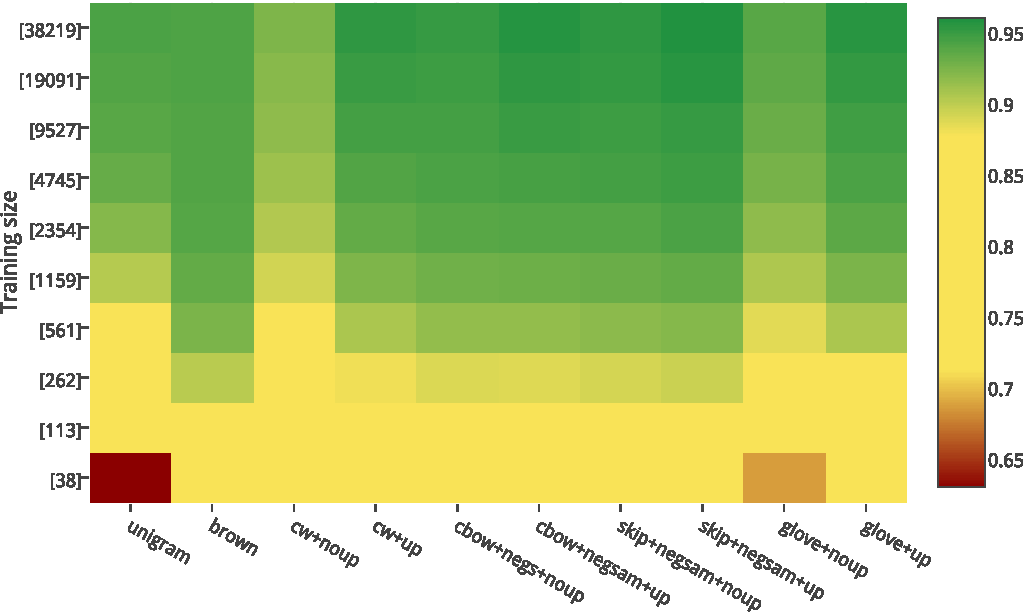
\includegraphics[scale=0.4]{plots/map-pos-color-invert.pdf}}\hfill
 \subfloat[Some other figure]{\includegraphics[width=0.48\textwidth]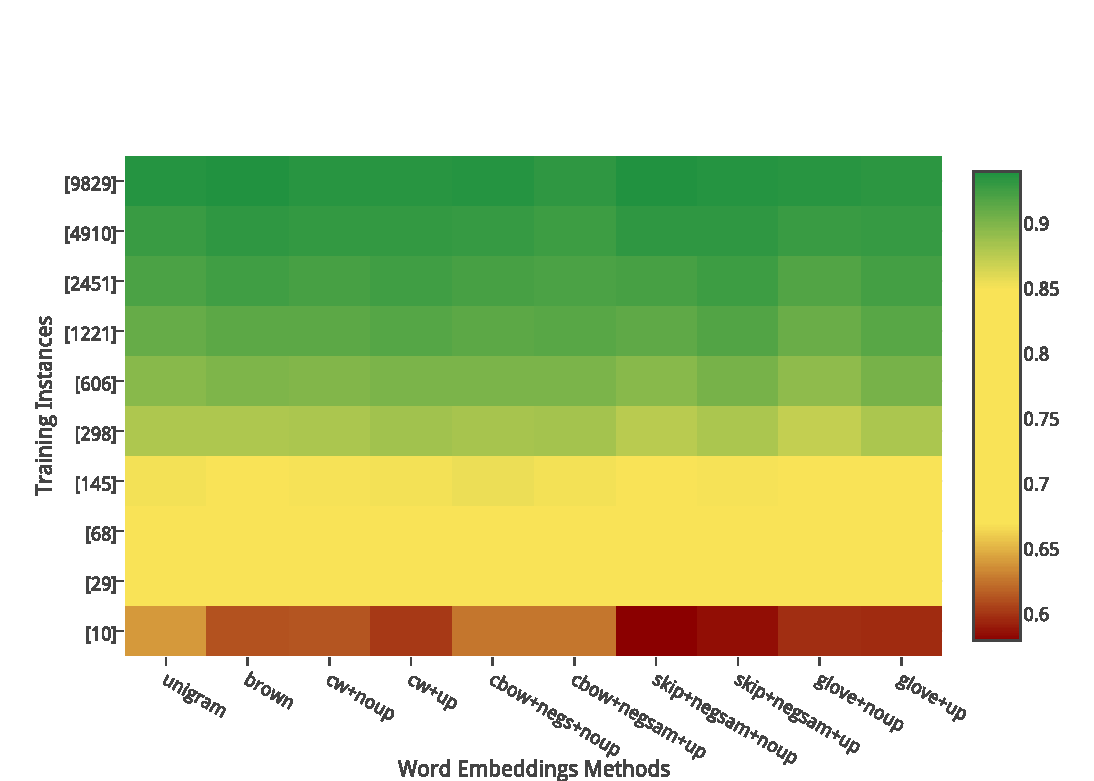
\includegraphics[scale=0.4]{plots/map-chunk-color-invert}}\\[-2ex]  %%<-- in this line
 \subfloat[Some more]{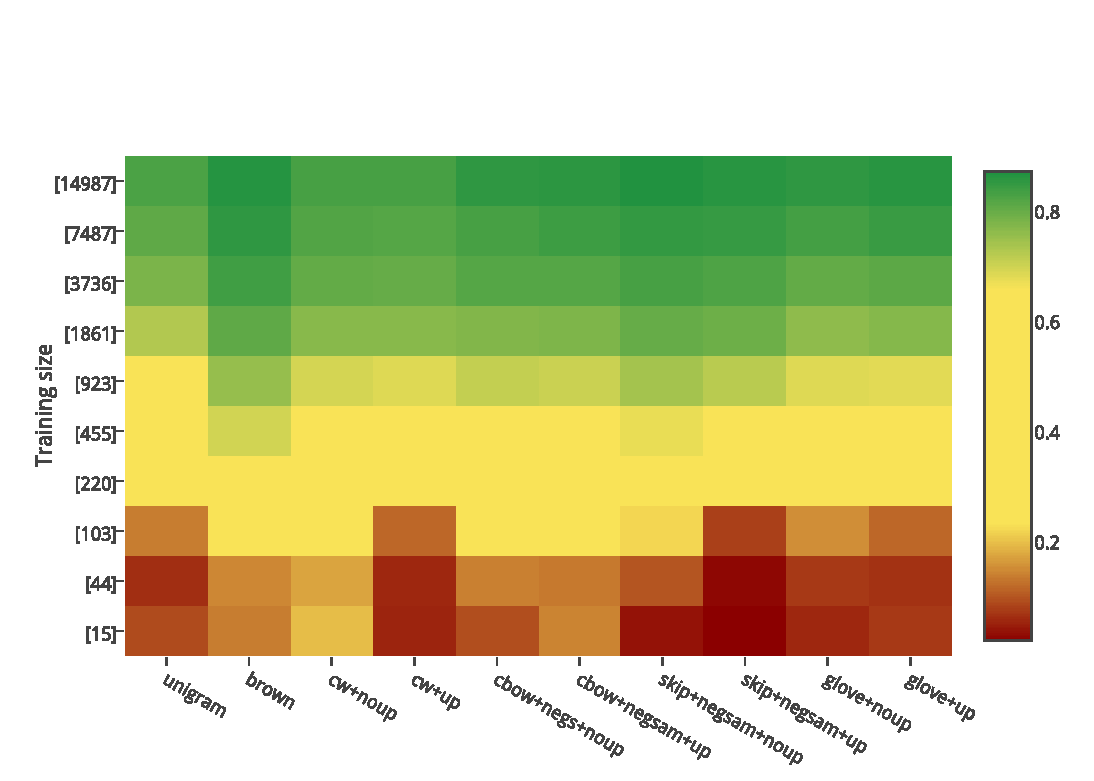
\includegraphics[scale=0.4]{plots/map-ner-color-invert}}\hfill
 \subfloat[Some less]{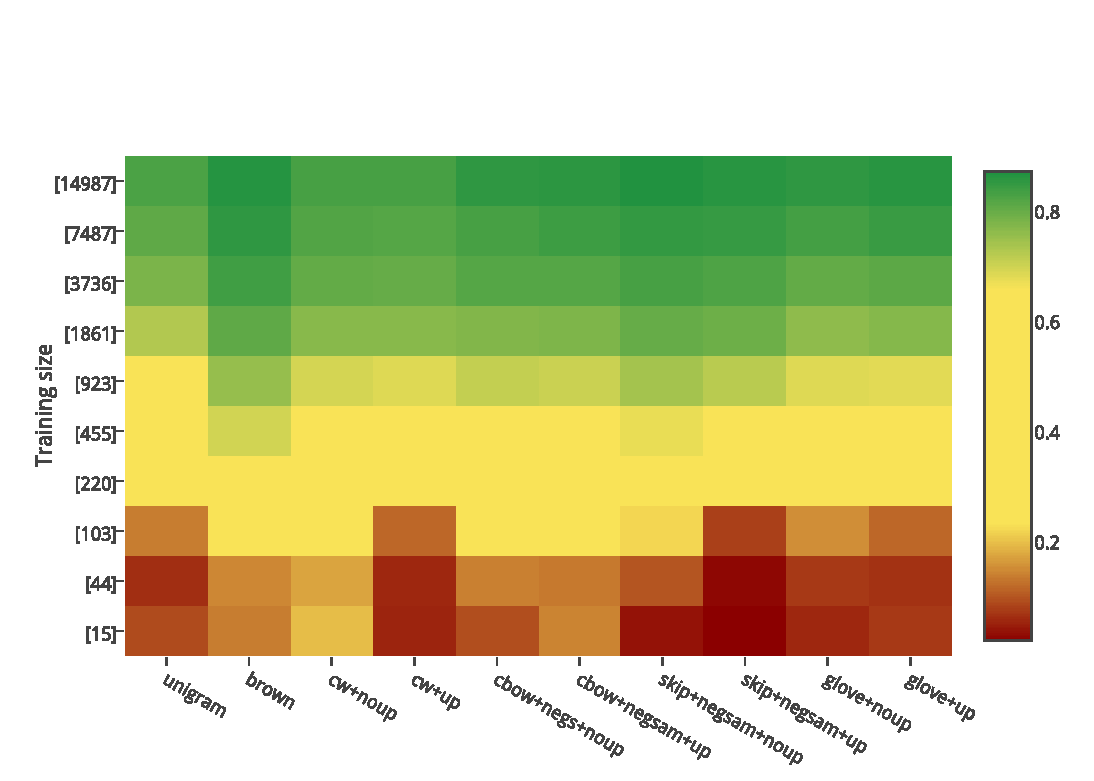
\includegraphics[scale=0.4]{plots/map-ner-color-invert}}
 \caption{There are example figures}
\end{figure}
\fi



%%%%%%%%%%%%%%%%%%%%%%%%%%%%
%%% OOV 
\begin{figure*}
\centering
\caption{Out-of-vocabulary-words (OOV) accuracy for \textit{in-domain} and \textit{out-of-domain} test sets}
\label{OOV} 
    	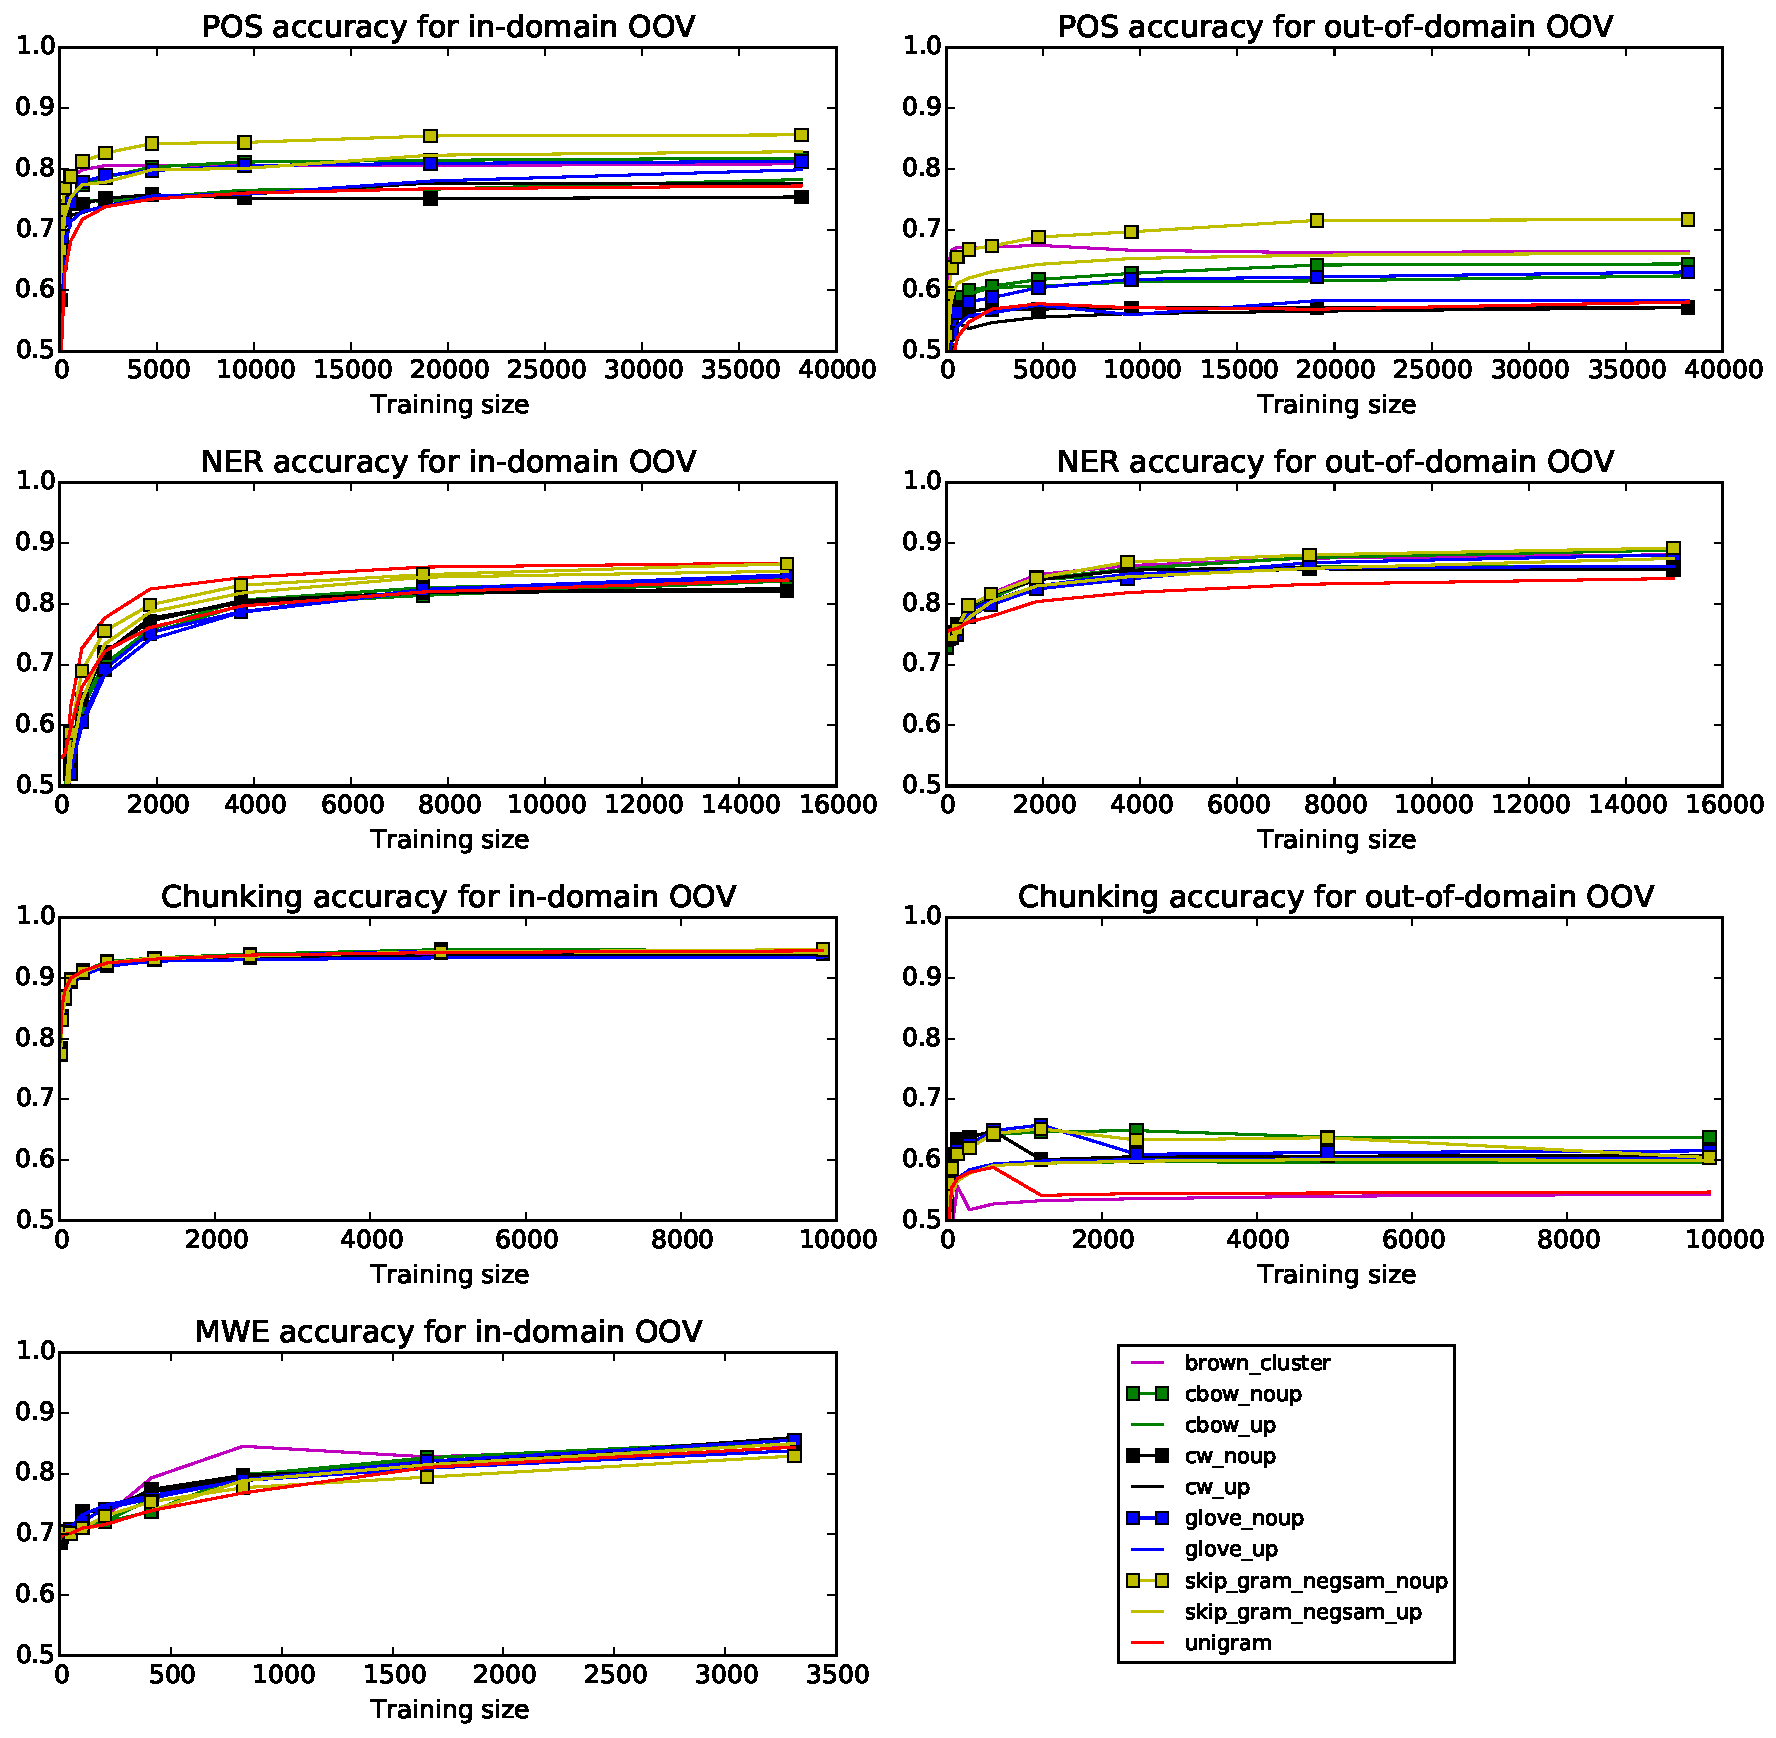
\includegraphics[scale=0.5]{plots/OOV-plots}
\end{figure*}








\section{Related Work}
%Word embedding learning methods have been applied to several 
%NLP tasks that we summaries in this section.

\newcite{collobert2011natural} proposed a unified neural network framework
that learns word embeddings and applied it to \pos, \chunking, \ner and semantic role labelling. 
When they combined word embeddings with hand-crafted features
(e.g., word suffixes for \pos;  gazetteers for \ner) and applied other
tricks like cascading and classifier combination, they achieved state-of-the-art performance.
% they system is very fast too.
Similarly, \newcite{turian2010word} evaluated three different word representations on \ner and \chunking, and concluded that unsupervised word representations improved \ner and \chunking. They also found that combining different word representations can further improve performance. \newcite{guo2014revisiting} also explored different ways of using word embeddings for \ner.  \newcite{owoputi2013improved} and \newcite{Schneider+:2014} found that \brown clustering enhances Twitter POS tagging and \mwe, respectively. Compared to previous work, we consider \textit{more} word representations including the most recent work and evaluate them on \textit{more} sequence labelling tasks, wherein the models are trained with training sets of varying size.

\newcite{Bansal+:2014} reported that direct use of word embeddings in dependency parsing did not show improvement. They achieved an improvement only when they performed hierarchical clustering of the word embeddings, and used features extracted from the cluster hierarchy.
In a similar vein, \newcite{Andreas:Klein:2014} explored the use of word embeddings for constituency parsing and concluded that the
information contained in word embeddings might duplicate the one acquired by a
syntactic parser, unless the training set is extremely small.
Other syntactic parsing studies that reported improvements by using
word embeddings include \newcite{Koo:2008}, \newcite{Koo:2010},
\newcite{Haffari:2011}, \newcite{Tratz:2011} and \newcite{chen:2014}.

Word embeddings have also been applied to other (non-sequential NLP)
tasks like grammar induction \cite{Spitkovsky:2011}, and semantic tasks
such as semantic relatedness, synonymy detection, concept
categorisation, selectional preference learning and analogy \cite{baroni:2014,Levy:2014,Levy:2015}.

\newcite{Huang:2009} demonstrated that using distributional word representations methods (like TF-IDF and LSA) as features, improves the labelling of OOV, when test for \pos and \chunking. In our study, we evaluate the labelling performance of OOV words for updated vs.\ non-updated word embedding representations, relative to the training set and with out-of-domain data.



%\nss{[Guo et al. 2014?]}

% such as super-sense tagging \cite{Grave:2013};

% Koo, T., Carreras, X., & Collins, M. (2008). Simple semi-supervised dependency parsing. ACL (pp. 595?603).
% Koo et al., 2008; http://cs.nyu.edu/~dsontag/papers/KooEtAl_emnlp10.pdf Dual Decomposition for Parsing with Non-Projective Head Automata - Dependency parsing.

%Haffari et al., 2011; http://www.aclweb.org/anthology/P11-2125 Ensemble of different dependency parsing models, each model corresponding to a different syntactic/semantic word clustering annotation.

% Supersense tagger (Grave et al., 2013) https://hal.inria.fr/hal-00833288/PDF/final-version.pdf

%%% Local Variables: 
%%% mode: latex
%%% TeX-PDF-mode: t 
%%% TeX-master: "WordEmbEvaluation"
%%% End: 

\section{Conclusions}

We have performed an extensive extrinsic evaluation of five word embedding methods
under fixed experimental conditions, and evaluated their applicability to four sequence tagging tasks: \pos, \chunking, \ner and \mwe identification.
We found that word embedding features reliably outperformed unigram
features, especially with limited training data, but that there was
relatively little difference over Brown clusters, and
no one embedding method was consistently superior across the different tasks and settings.
Word embeddings and Brown clusters were also found to improve
out-of-domain performance and for OOV words.
We expected a performance gap between the fixed and task-updated embeddings, but the observed difference was marginal.
Indeed, we found that updating can result in overfitting.
We also carried out preliminary analysis of the impact of updating on
the vectors, a direction which we intend to pursue further.

% Finally, by using word embeddings as features for MWE identification, we outperformed 
% the state-of-the-art system on that task.
% %We could not find any trend that suggest that a word embedding method is better than other.
% We hope to build on this in future work by learning representations directly over multiword units.\nss{[Has there been any research into this issue?]}


%%% Local Variables: 
%%% mode: latex
%%% TeX-PDF-mode: t 
%%% TeX-master: "WordEmbEvaluation"
%%% End: 


% \section*{Acknowledgments}

% Anonymised\\
% Anonymised\\
% Anonymised\\
% Anonymised\\
% Anonymised\\
% Anonymised\\

%NICTA is funded by the Australian Government as represented by the Department of Broadband, Communications and the Digital Economy and the Australian Research Council through the ICT Centre of Excellence program.

\bibliographystyle{acl2013}
\bibliography{biblio}

\end{document}


%%% Local Variables: 
%%% mode: latex
%%% TeX-PDF-mode: t 
%%% TeX-master: t
%%% End: 
